    
    \hypertarget{qubits-to-linear-algebra-mathematical-toolkit}{%
\section{Jupyter Notebook Unit 2.1 - 2.3: Qubits to Linear Algebra Mathematical~Toolkit}\label{qubits-to-linear-algebra-mathematical-toolkit}}

\emph{(building directly on § 1.2~``Qubit representations~\& mainstream
hardware'')}

\begin{longtable}[]{@{}
  >{\raggedright\arraybackslash}p{(\columnwidth - 2\tabcolsep) * \real{0.4000}}
  >{\raggedright\arraybackslash}p{(\columnwidth - 2\tabcolsep) * \real{0.6000}}@{}}
\toprule\noalign{}
\begin{minipage}[b]{\linewidth}\raggedright
Code
\end{minipage} & \begin{minipage}[b]{\linewidth}\raggedright
Outcome
\end{minipage} \\
\midrule\noalign{}
\endhead
\bottomrule\noalign{}
\endlastfoot
2.0-A & \textbf{distinguish} a classical bit from a qubit in one
sentence. \\
2.0-B & \textbf{write} an arbitrary single-qubit pure state as
\(\lvert\psi\rangle=\alpha\lvert0\rangle+\beta\lvert1\rangle\) and
\textbf{explain} why
\(\lvert\alpha\lvert^2 + \lvert\beta\lvert^2 = 1\). \\
2.0-C & \textbf{compute} measurement probabilities and \textbf{plot} the
corresponding Bloch-sphere vector using the provided Python cell. \\
2.0-D & \textbf{interpret} latitude \((\theta)\) and longitude
\((\phi)\) angles on the Bloch sphere in terms of amplitudes. \\
\end{longtable}

\begin{center}\rule{0.5\linewidth}{0.5pt}\end{center}

\hypertarget{recap---from-physical-qubits-to-state-vectors}{%
\subsection*{2.0~Recap~-~From Physical Qubits to
State-Vectors}\label{recap---from-physical-qubits-to-state-vectors}}

\begin{quote}
How every physical qubit maps to a unit-norm vector in \(\mathbb C^{2}\)
and how the Bloch-sphere parameters \((\theta,\phi)\) encode amplitudes.

This abstraction lets us ignore hardware details and perform algorithm
design entirely in linear-algebra terms.
\end{quote}

\begin{figure}
\centering
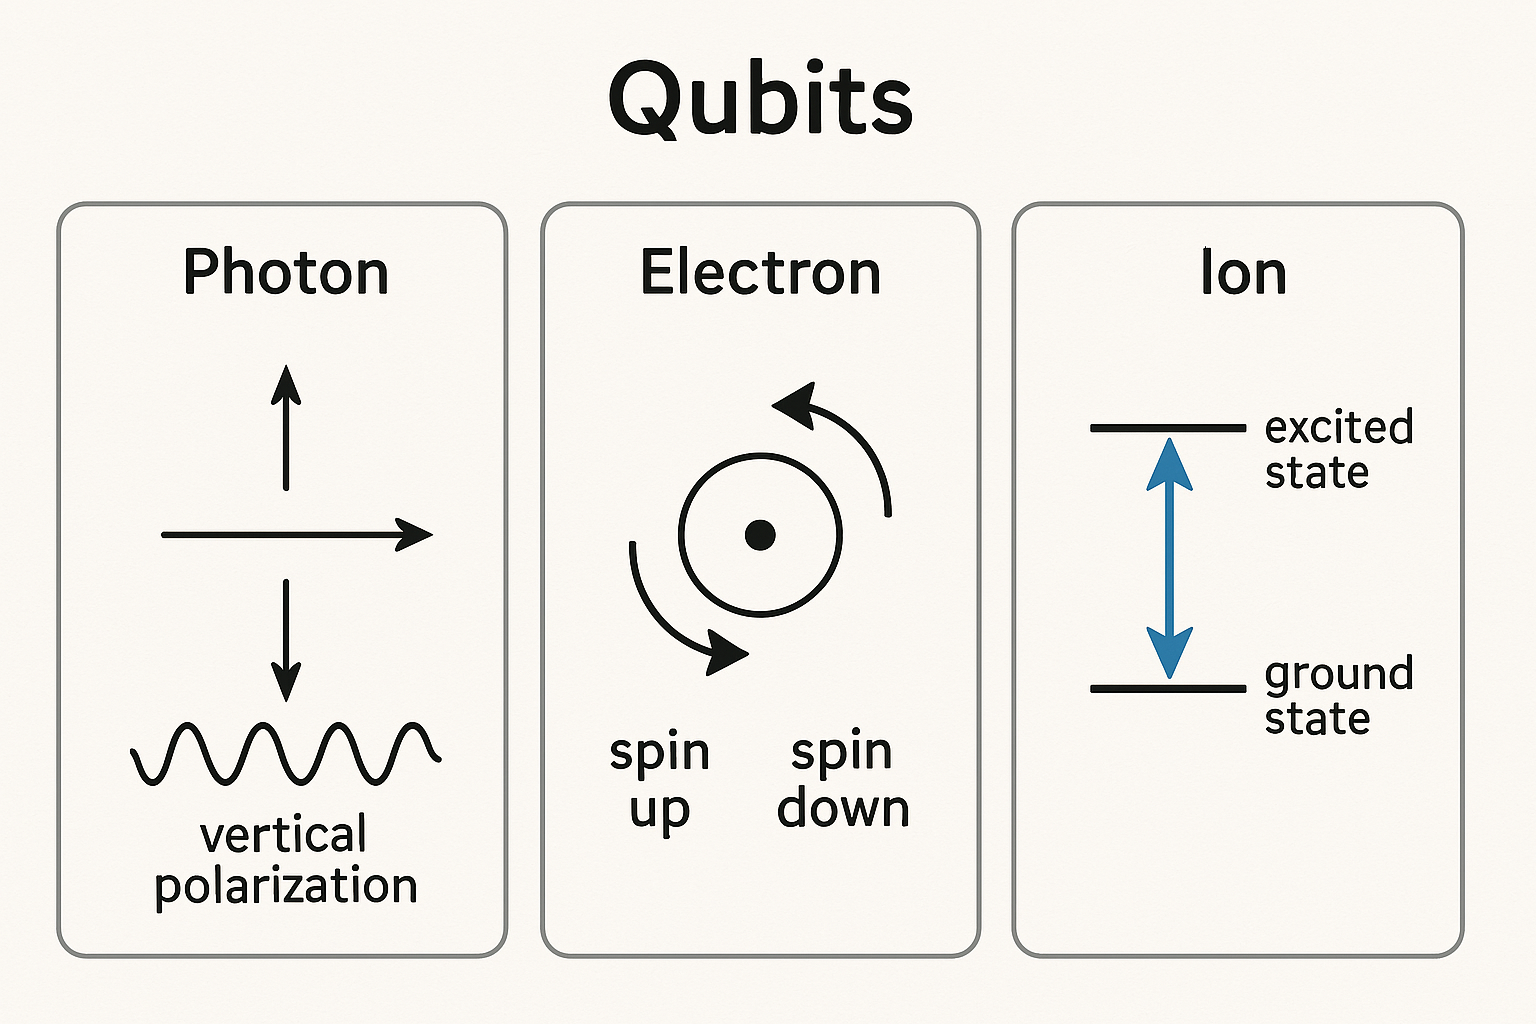
\includegraphics{figures/physical_qubits.png}
\caption{Physical Qubits}
\end{figure}

\begin{quote}
\textbf{Take-away:} physical implementation-ion-trap, superconducting,
photonic-can be abstracted as a \textbf{two-level quantum system} whose
logical states we call\\
\[
\lvert0\rangle,\; \lvert1\rangle .
\]
\end{quote}

\begin{itemize}
\tightlist
\item
  qubit is an analogous to classical bit;
\end{itemize}

\begin{longtable}[]{@{}
  >{\raggedright\arraybackslash}p{(\columnwidth - 2\tabcolsep) * \real{0.4000}}
  >{\raggedright\arraybackslash}p{(\columnwidth - 2\tabcolsep) * \real{0.6000}}@{}}
\toprule\noalign{}
\begin{minipage}[b]{\linewidth}\raggedright
Classical bit
\end{minipage} & \begin{minipage}[b]{\linewidth}\raggedright
Quantum bit (qubit)
\end{minipage} \\
\midrule\noalign{}
\endhead
\bottomrule\noalign{}
\endlastfoot
stores 0 \emph{or}~1 & stores a \textbf{state-vector} in
\(\mathbb C^{2}\) :
\(\displaystyle \lvert\psi\rangle=\alpha\lvert0\rangle+\beta\lvert1\rangle\) \\
operations are Boolean gates & operations are \textbf{unitaries}
(reversible 2×2 matrices) \\
\end{longtable}

\begin{center}\rule{0.5\linewidth}{0.5pt}\end{center}

\hypertarget{single-qubit-pure-state}{%
\subsubsection*{Single-qubit pure state}\label{single-qubit-pure-state}}

Quantum systems have states, and for a qubit those orthogonal states are
\( \lvert0\rangle\) and \(\lvert1\rangle \) {[}using ket notation{]}.

\begin{itemize}
\item
  \(\lvert0\rangle\) and \(\lvert1\rangle\) are known as the
  \emph{computational basis} states.
\item
  It is possible to have linear combinations of states, called
  \emph{superpositions} where \(\alpha\) \& \(\beta\) are complex
  values:

  \[|\psi\rangle = \alpha \lvert0\rangle + \beta \lvert1\rangle\]
\item
  \(\lvert0\rangle\) and \(\lvert1\rangle\) form an ortho-normal basis
  for the qubit 2-dimensional complex vector space.
\end{itemize}

\begin{center}\rule{0.5\linewidth}{0.5pt}\end{center}

\hypertarget{measurement-probabilities}{%
\subsubsection*{Measurement
Probabilities}\label{measurement-probabilities}}

\(\alpha\) \& \(\beta\) are (complex valued) amplitudes which give the
measurement probability on obtaining a basis outcome \(\lvert0\rangle\)
or \(\lvert1\rangle\).

\begin{itemize}
\item
  \(P(\lvert0\rangle) = \lvert\alpha\lvert^2 \quad P(\lvert1\rangle) = \lvert\beta\lvert^2\)
  \textgreater{} For a pure state of a 3 qubit register, the probability
  of measuring one basis state would be: \textgreater{} \textgreater{}
   \( P(\lvert010\rangle) = \lvert\alpha\_1\beta\_2\alpha\_3\lvert\^{}2 \)
\item
  The sum of probabilities of each of the basis outcomes must be 1,
  making the state a unit vector.
\item
  The quantum system is \emph{completely described} by this unit vector
  in the state space, its state-vector.

  \begin{quote}
  So the pure state \(\lvert\psi\rangle\) of a qubit is a unit vector in
  a 2-D complex vector space (actually \emph{Hilbert} space, we see
  later).

  \( \textbar{}\alpha\textbar\^{}2 + \textbar{}\beta\textbar\^{}2 =
  1 \rightarrow \) the state-vector is \textbf{unit-norm}.
  \end{quote}
\end{itemize}

\begin{center}\rule{0.5\linewidth}{0.5pt}\end{center}

\hypertarget{bloch-sphere-picture}{%
\subsubsection*{Bloch-sphere picture}\label{bloch-sphere-picture}}

All single-qubit pure states live on the unit sphere in
\(\mathbb C^{3}\):

\[
\lvert\psi\rangle
=\cos\frac{\theta}{2}\,\lvert0\rangle
+\;e^{i\varphi}\sin\frac{\theta}{2}\,\lvert1\rangle ,
\quad
0\le\theta\le\pi,\;0\le\varphi<2\pi .
\]

\begin{figure}
\centering
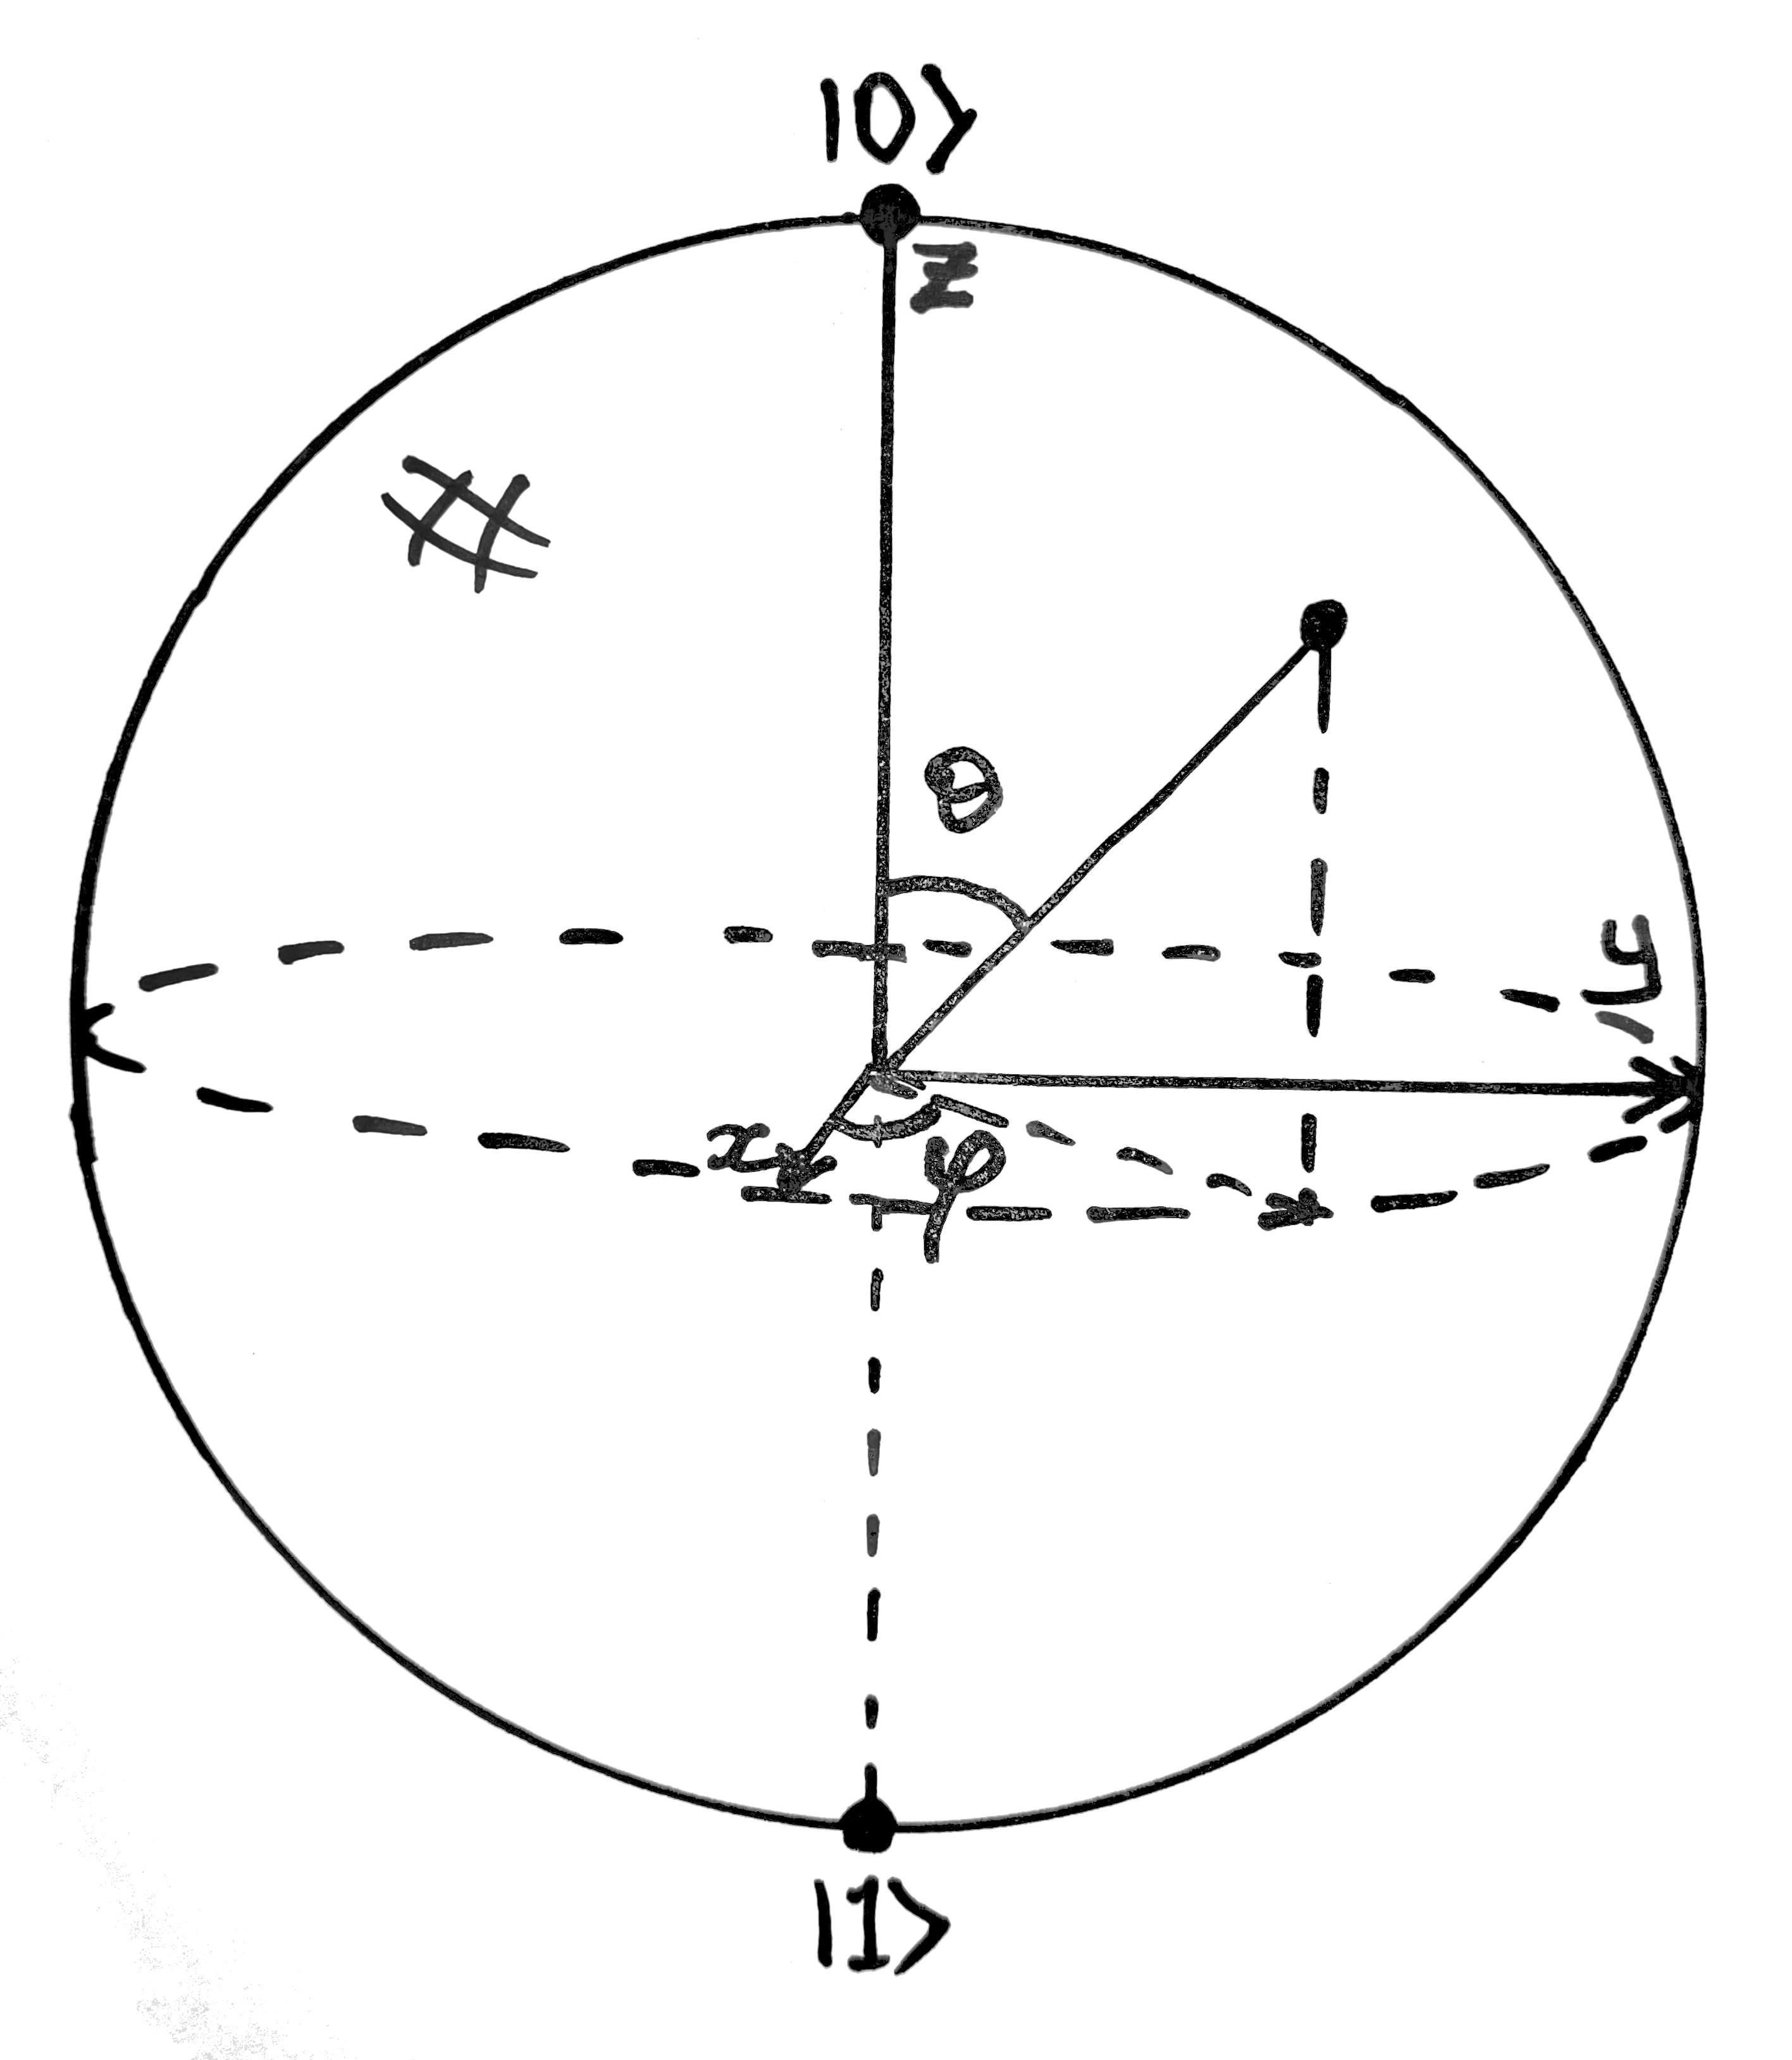
\includegraphics{figures/blochsphere.png}
\caption{Bloch sphere annotated}
\end{figure}

\begin{quote}
\emph{create a Bloch vector for \(\theta=\pi/3,\;\phi=\pi/2\) and plot
it.}
\end{quote}

    \begin{tcolorbox}[breakable, size=fbox, boxrule=1pt, pad at break*=1mm,colback=cellbackground, colframe=cellborder]
\prompt{In}{incolor}{1}{\boxspacing}
\begin{Verbatim}[commandchars=\\\{\}]
\PY{k+kn}{import} \PY{n+nn}{numpy} \PY{k}{as} \PY{n+nn}{np}
\PY{k+kn}{from} \PY{n+nn}{qiskit}\PY{n+nn}{.}\PY{n+nn}{visualization} \PY{k+kn}{import} \PY{n}{plot\PYZus{}bloch\PYZus{}vector}

\PY{n}{theta}\PY{p}{,} \PY{n}{phi} \PY{o}{=} \PY{n}{np}\PY{o}{.}\PY{n}{pi}\PY{o}{/}\PY{l+m+mi}{3}\PY{p}{,} \PY{n}{np}\PY{o}{.}\PY{n}{pi}\PY{o}{/}\PY{l+m+mi}{2}
\PY{n}{bloch\PYZus{}vec} \PY{o}{=} \PY{p}{[}\PY{n}{np}\PY{o}{.}\PY{n}{sin}\PY{p}{(}\PY{n}{theta}\PY{p}{)}\PY{o}{*}\PY{n}{np}\PY{o}{.}\PY{n}{cos}\PY{p}{(}\PY{n}{phi}\PY{p}{)}\PY{p}{,}   \PY{c+c1}{\PYZsh{} x}
             \PY{n}{np}\PY{o}{.}\PY{n}{sin}\PY{p}{(}\PY{n}{theta}\PY{p}{)}\PY{o}{*}\PY{n}{np}\PY{o}{.}\PY{n}{sin}\PY{p}{(}\PY{n}{phi}\PY{p}{)}\PY{p}{,}   \PY{c+c1}{\PYZsh{} y}
             \PY{n}{np}\PY{o}{.}\PY{n}{cos}\PY{p}{(}\PY{n}{theta}\PY{p}{)}\PY{p}{]}               \PY{c+c1}{\PYZsh{} z}
\PY{n}{plot\PYZus{}bloch\PYZus{}vector}\PY{p}{(}\PY{n}{bloch\PYZus{}vec}\PY{p}{)}
\end{Verbatim}
\end{tcolorbox}
 
            
\prompt{Out}{outcolor}{1}{}
    
    \begin{center}
    \adjustimage{max size={0.9\linewidth}{0.9\paperheight}}{figures/unit_2.0_from-qubits-to-linear-algebra_1_0.png}
    \end{center}
    { \hspace*{\fill} \\}
    

    \hypertarget{dirac-notation-multiqubit-basis}{%
\subsection*{2.1\,Dirac Notation \& Multi‑Qubit
Basis}\label{dirac-notation-multiqubit-basis}}

Compact bra‑ket language and the \(2^{n}\)-dimensional computational
basis for \(n\) qubits.

Provides the shorthand used in all quantum‑algorithm papers and allows
us to label, index and program multi‑qubit circuits unambiguously.

\begin{longtable}[]{@{}
  >{\raggedright\arraybackslash}p{(\columnwidth - 2\tabcolsep) * \real{0.4000}}
  >{\raggedright\arraybackslash}p{(\columnwidth - 2\tabcolsep) * \real{0.6000}}@{}}
\toprule\noalign{}
\begin{minipage}[b]{\linewidth}\raggedright
Code
\end{minipage} & \begin{minipage}[b]{\linewidth}\raggedright
Outcome
\end{minipage} \\
\midrule\noalign{}
\endhead
\bottomrule\noalign{}
\endlastfoot
\,2.1‑A & \textbf{translate} between column‑vector and
\(\lvert\cdot\rangle\) notation for any 2‑component state. \\
\,2.1‑B & \textbf{enumerate} all \(2^{n}\) computational basis states
for \(n\le 3\) and \textbf{state} the dimension of the Hilbert space. \\
\,2.1‑C & \textbf{normalise} a given two‑qubit amplitude list and
\textbf{verify} the norm with Python. \\
\end{longtable}

\begin{center}\rule{0.5\linewidth}{0.5pt}\end{center}

\hypertarget{kets-and-bras}{%
\paragraph{Kets and Bras}\label{kets-and-bras}}

A \textbf{ket} is a column vector

\[
\lvert\psi\rangle \;=\;
\begin{pmatrix}
\psi_0 \\ \psi_1 \\ \vdots \\ \psi_{d-1}
\end{pmatrix},
\] while its \textbf{bra} is the conjugate‑transpose (row)\\
\[
\langle\psi\lvert \;=\;
\bigl(\psi_0^{\!*},\;\psi_1^{\!*},\;\dots,\;\psi_{d-1}^{\!*}\bigr).
\]

\begin{center}\rule{0.5\linewidth}{0.5pt}\end{center}

\hypertarget{computational-basis}{%
\paragraph{Computational basis}\label{computational-basis}}

Dirac notation uses bit strings \(\{0,1\}^n\) (e.g.~\(\lvert0\rangle\)
and \(\lvert1\rangle\))

\begin{itemize}
\tightlist
\item
  For \(n\) qubits the \emph{computational (standard) basis} is\\
  \textgreater{}
  \(\bigl\{\;\lvert x\rangle : x\in\{0,1\}^{\,n}\bigr\},\)
  \textgreater{} \textgreater{} a set of \(2^{n}\) mutually orthonormal
  vectors. \textgreater{} \textgreater{} If \(n = 3\), one standard
  basis is \(\lvert011\rangle\), and \(\langle011\lvert\) is the row
  vector: \((00010000)\).
\end{itemize}

\begin{center}\rule{0.5\linewidth}{0.5pt}\end{center}

\hypertarget{example---two-qubits}{%
\paragraph{Example - two qubits}\label{example---two-qubits}}

A general pure state of two qubits is

\[
\lvert\phi\rangle \;=\;
\alpha_{00}\lvert 00\rangle + 
\alpha_{01}\lvert 01\rangle + 
\alpha_{10}\lvert 10\rangle + 
\alpha_{11}\lvert 11\rangle
\] \[
\qquad
\|\phi\|^{2}
=\sum_{i,j\in\{0,1\}} |\alpha_{ij}|^{2}=1 .
\]

    \begin{tcolorbox}[breakable, size=fbox, boxrule=1pt, pad at break*=1mm,colback=cellbackground, colframe=cellborder]
\prompt{In}{incolor}{2}{\boxspacing}
\begin{Verbatim}[commandchars=\\\{\}]
\PY{c+c1}{\PYZsh{}\PYZsh{}\PYZsh{}\PYZsh{} Quick Python check \PYZhy{} normalise a random two\PYZhy{}qubit state}
\PY{k+kn}{import} \PY{n+nn}{numpy} \PY{k}{as} \PY{n+nn}{np}

\PY{c+c1}{\PYZsh{} random complex amplitudes}
\PY{n}{amps} \PY{o}{=} \PY{n}{np}\PY{o}{.}\PY{n}{random}\PY{o}{.}\PY{n}{randn}\PY{p}{(}\PY{l+m+mi}{4}\PY{p}{)} \PY{o}{+} \PY{l+m+mi}{1}\PY{n}{j}\PY{o}{*}\PY{n}{np}\PY{o}{.}\PY{n}{random}\PY{o}{.}\PY{n}{randn}\PY{p}{(}\PY{l+m+mi}{4}\PY{p}{)}
\PY{n}{phi}  \PY{o}{=} \PY{n}{amps} \PY{o}{/} \PY{n}{np}\PY{o}{.}\PY{n}{linalg}\PY{o}{.}\PY{n}{norm}\PY{p}{(}\PY{n}{amps}\PY{p}{)}          \PY{c+c1}{\PYZsh{} normalise}

\PY{n+nb}{print}\PY{p}{(}\PY{l+s+s2}{\PYZdq{}}\PY{l+s+s2}{State vector |φ⟩ =}\PY{l+s+s2}{\PYZdq{}}\PY{p}{,} \PY{n}{phi}\PY{p}{)}
\PY{n+nb}{print}\PY{p}{(}\PY{l+s+s2}{\PYZdq{}}\PY{l+s+s2}{Norm² =}\PY{l+s+s2}{\PYZdq{}}\PY{p}{,} \PY{n}{np}\PY{o}{.}\PY{n}{vdot}\PY{p}{(}\PY{n}{phi}\PY{p}{,} \PY{n}{phi}\PY{p}{)}\PY{o}{.}\PY{n}{real}\PY{p}{)}    \PY{c+c1}{\PYZsh{} should print 1.0}
\end{Verbatim}
\end{tcolorbox}

    \begin{Verbatim}[commandchars=\\\{\}]
State vector |φ⟩ = [-0.73202702-0.03449025j -0.20235518+0.3679845j
0.10864371-0.09399594j
  0.49096349-0.15780625j]
Norm² = 1.0
    \end{Verbatim}

    \hypertarget{vector-spaces-refresher}{%
\subsection*{2.2\,Vector Spaces
Refresher}\label{vector-spaces-refresher}}

Addition, scalar multiplication, spanning sets, linear independence, and
what a \emph{basis} really is.

These are the axioms under every quantum proof; without them you can't
talk about dimensions, change‑of‑basis, or well‑posed linear systems.

\begin{longtable}[]{@{}
  >{\raggedright\arraybackslash}p{(\columnwidth - 2\tabcolsep) * \real{0.4000}}
  >{\raggedright\arraybackslash}p{(\columnwidth - 2\tabcolsep) * \real{0.6000}}@{}}
\toprule\noalign{}
\begin{minipage}[b]{\linewidth}\raggedright
Code
\end{minipage} & \begin{minipage}[b]{\linewidth}\raggedright
Outcome
\end{minipage} \\
\midrule\noalign{}
\endhead
\bottomrule\noalign{}
\endlastfoot
\,2.2‑A & \textbf{perform} vector addition and scalar multiplication on
complex \(n\)-tuples in code. \\
\,2.2‑B & \textbf{identify} whether a provided set of vectors in
\(\mathbb C^{n}\) is linearly independent. \\
\,2.2‑C & \textbf{express} \(\lvert0\rangle,\lvert1\rangle\) as explicit
column matrices and \textbf{show} they form a basis of
\(\mathbb C^{2}\). \\
\end{longtable}

\begin{center}\rule{0.5\linewidth}{0.5pt}\end{center}

\hypertarget{complex-vector-space-addition-and-scalar-multiplication}{%
\paragraph{Complex Vector Space Addition and Scalar
multiplication}\label{complex-vector-space-addition-and-scalar-multiplication}}

A complex vector space \textbf{vector space} V over \(\mathbb C\) of
dimension \(n\), \(V=C^n\), is the set\\
\[
\mathbb C^{\,n}\;=\;\bigl\{(z_{1},\dots,z_{n})^{T}\;|\;z_k\in\mathbb C\bigr\},
\] equipped with

\begin{itemize}
\item
  \textbf{Addition}\\
  \[
  (v+w)_k \;=\; v_k + w_k ,
  \]
\item
  \textbf{Scalar multiplication}\\
  \[
  (\lambda v)_k \;=\; \lambda\,v_k ,\quad \lambda\in\mathbb C .
  \]
\end{itemize}

The \textbf{zero vector} \(0=(0,\dots,0)^{T}\) satisfies \(v+0=v\).

\begin{itemize}
\item
  \textbf{Zero vector} \(0\) has all elements as 0: \((0, 0, ... , 0)\)
\item
  \textbf{Zero element}
\end{itemize}

\begin{center}\rule{0.5\linewidth}{0.5pt}\end{center}

\hypertarget{spanning-sets-bases}{%
\paragraph{Spanning Sets \& Bases}\label{spanning-sets-bases}}

A list of vectors \(\{v_1,\dots,v_m\}\subseteq\mathbb C^{n}\)

\begin{itemize}
\tightlist
\item
  \textbf{spans} the space if every \(u\in\mathbb C^{n}\) can be
  written\\
  \(u=\sum_{j=1}^{m} \alpha_j v_j\).\\
\item
  is \textbf{linearly independent} if \(\sum\alpha_j v_j = 0\) implies
  all \(\alpha_j=0\).
\end{itemize}

If it both spans and is independent, it is a \textbf{basis}; any basis
of \(\mathbb C^{n}\) contains exactly \(n\) vectors.

\begin{center}\rule{0.5\linewidth}{0.5pt}\end{center}

\hypertarget{singlequbit-example}{%
\paragraph{Single‑Qubit Example}\label{singlequbit-example}}

For one qubit, the matrix representation the computational--basis kets,
\(\lvert0\rangle\) and \(\lvert1\rangle\), are: \[
\lvert0\rangle=\begin{pmatrix}1\\0\end{pmatrix},
\quad
\lvert1\rangle=\begin{pmatrix}0\\1\end{pmatrix}
\]

\begin{itemize}
\item
  They span \(\mathbb C^{2}\)
\item
  Are independent because neither row elements sum to zero:
  \(1 + 0 = 1\) and \(0 + 1 = 1\)
\item
  Therefore form a basis.
\end{itemize}

\begin{center}\rule{0.5\linewidth}{0.5pt}\end{center}

    \begin{tcolorbox}[breakable, size=fbox, boxrule=1pt, pad at break*=1mm,colback=cellbackground, colframe=cellborder]
\prompt{In}{incolor}{3}{\boxspacing}
\begin{Verbatim}[commandchars=\\\{\}]
\PY{c+c1}{\PYZsh{}\PYZsh{}\PYZsh{}\PYZsh{} Python demo \PYZhy{} linear independence test}
\PY{k+kn}{import} \PY{n+nn}{numpy} \PY{k}{as} \PY{n+nn}{np}

\PY{n}{e0} \PY{o}{=} \PY{n}{np}\PY{o}{.}\PY{n}{array}\PY{p}{(}\PY{p}{[}\PY{l+m+mi}{1}\PY{p}{,}\PY{l+m+mi}{0}\PY{p}{]}\PY{p}{)}
\PY{n}{e1} \PY{o}{=} \PY{n}{np}\PY{o}{.}\PY{n}{array}\PY{p}{(}\PY{p}{[}\PY{l+m+mi}{0}\PY{p}{,}\PY{l+m+mi}{1}\PY{p}{]}\PY{p}{)}
\PY{n}{M}  \PY{o}{=} \PY{n}{np}\PY{o}{.}\PY{n}{column\PYZus{}stack}\PY{p}{(}\PY{p}{[}\PY{n}{e0}\PY{p}{,} \PY{n}{e1}\PY{p}{]}\PY{p}{)}   \PY{c+c1}{\PYZsh{} 2×2 matrix whose columns are the vectors}

\PY{n}{rank} \PY{o}{=} \PY{n}{np}\PY{o}{.}\PY{n}{linalg}\PY{o}{.}\PY{n}{matrix\PYZus{}rank}\PY{p}{(}\PY{n}{M}\PY{p}{)}
\PY{n+nb}{print}\PY{p}{(}\PY{l+s+s2}{\PYZdq{}}\PY{l+s+s2}{Rank =}\PY{l+s+s2}{\PYZdq{}}\PY{p}{,} \PY{n}{rank}\PY{p}{,} \PY{l+s+s2}{\PYZdq{}}\PY{l+s+s2}{ (basis)}\PY{l+s+s2}{\PYZdq{}} \PY{k}{if} \PY{n}{rank}\PY{o}{==}\PY{l+m+mi}{2} \PY{k}{else} \PY{l+s+s2}{\PYZdq{}}\PY{l+s+s2}{ (not independent)}\PY{l+s+s2}{\PYZdq{}}\PY{p}{)}

\PY{c+c1}{\PYZsh{} Verify in Python that X ∣0⟩=∣1⟩X∣0⟩=∣1⟩.}
\PY{n}{X} \PY{o}{=} \PY{n}{np}\PY{o}{.}\PY{n}{array}\PY{p}{(}\PY{p}{[}\PY{p}{[}\PY{l+m+mi}{0}\PY{p}{,}\PY{l+m+mi}{1}\PY{p}{]}\PY{p}{,}\PY{p}{[}\PY{l+m+mi}{1}\PY{p}{,}\PY{l+m+mi}{0}\PY{p}{]}\PY{p}{]}\PY{p}{)}
\PY{n+nb}{print}\PY{p}{(}\PY{l+s+s2}{\PYZdq{}}\PY{l+s+s2}{X}\PY{l+s+s2}{\PYZbs{}}\PY{l+s+s2}{lvert0}\PY{l+s+se}{\PYZbs{}r}\PY{l+s+s2}{angle =}\PY{l+s+s2}{\PYZdq{}}\PY{p}{,} \PY{n}{X}\PY{o}{.}\PY{n}{dot}\PY{p}{(}\PY{n}{e0}\PY{p}{)}\PY{p}{)}
\end{Verbatim}
\end{tcolorbox}

    \begin{Verbatim}[commandchars=\\\{\}]
Rank = 2  (basis)
angle = [0 1]
    \end{Verbatim}

    \hypertarget{linear-operators-pauli-friends}{%
\subsection*{2.3\,Linear Operators (Pauli \&
Friends)}\label{linear-operators-pauli-friends}}

Definition of a linear operator, identity/zero maps, and the Pauli
matrices as elementary single‑qubit unitaries.

Gates \emph{are} linear operators; mastering Pauli algebra is
prerequisite for circuit decomposition, error correction and Hamiltonian
simulation.

\begin{longtable}[]{@{}
  >{\raggedright\arraybackslash}p{(\columnwidth - 2\tabcolsep) * \real{0.4000}}
  >{\raggedright\arraybackslash}p{(\columnwidth - 2\tabcolsep) * \real{0.6000}}@{}}
\toprule\noalign{}
\begin{minipage}[b]{\linewidth}\raggedright
Code
\end{minipage} & \begin{minipage}[b]{\linewidth}\raggedright
Outcome
\end{minipage} \\
\midrule\noalign{}
\endhead
\bottomrule\noalign{}
\endlastfoot
\,2.3‑A & \textbf{verify} line‑arity of a given matrix function \(A(v)\)
by symbolic or numeric test. \\
\,2.3‑B & \textbf{construct} the Pauli matrices in NumPy and
\textbf{demonstrate} \(X^{2}=Y^{2}=Z^{2}=I\). \\
\,2.3‑C & \textbf{explain} in ≤\,3 sentences why single‑qubit gates must
be unitary (linking to reversibility). \\
\end{longtable}

\begin{center}\rule{0.5\linewidth}{0.5pt}\end{center}

\hypertarget{what-is-a-linear-operator}{%
\paragraph{What is a Linear Operator?}\label{what-is-a-linear-operator}}

\begin{itemize}
\tightlist
\item
  linear operator as a function mapping vector spaces V -\textgreater{}
  W;
\end{itemize}

A map \(A : V \rightarrow V\) on a vector space \(V\) is \textbf{linear}
if\\
\[
A\bigl(\lambda v + w\bigr) \;=\; \lambda\,A v + A w
\qquad\forall\, v,w\in V,\;\lambda\in\mathbb C .
\]

\begin{itemize}
\item
  \textbf{Identity operator} \(I\) satisfies \(I v = v\).
\item
  Identity matrix:
\item
  \textbf{Zero operator} \(0\) maps a vector to zero vector and
  satisfies \(0 v = 0\).
\end{itemize}

\begin{center}\rule{0.5\linewidth}{0.5pt}\end{center}

\hypertarget{singlequbit-pauli-set}{%
\paragraph{Single‑Qubit Pauli Set}\label{singlequbit-pauli-set}}

\[
I \;=\;
\begin{pmatrix}
1 & 0 \\
0 & 1
\end{pmatrix},
\quad
X \;=\;
\begin{pmatrix}
0 & 1 \\
1 & 0
\end{pmatrix},
\quad
Y \;=\;
\begin{pmatrix}
0 & -i \\
i & 0
\end{pmatrix},
\quad
Z \;=\;
\begin{pmatrix}
1 & 0 \\
0 & -1
\end{pmatrix}.
\]

\begin{itemize}
\tightlist
\item
  \textbf{Hermitian}: \(P^\dagger = P\).\\
\item
  \textbf{Unitary}: \(P^\dagger P = I\).\\
\item
  \textbf{Squares to identity}: \(P^{2}=I\).
\end{itemize}

These four matrices plus overall phases generate all single‑qubit
unitaries.

\begin{center}\rule{0.5\linewidth}{0.5pt}\end{center}

\hypertarget{action-on-the-bloch-sphere}{%
\paragraph{Action on the Bloch
Sphere}\label{action-on-the-bloch-sphere}}

\begin{itemize}
\tightlist
\item
  \(X\)\,--- rotation by \(\pi\) around the \textbf{x‑axis}\\
\item
  \(Y\)\,--- rotation by \(\pi\) around the \textbf{y‑axis}\\
\item
  \(Z\)\,--- rotation by \(\pi\) around the \textbf{z‑axis}
\end{itemize}

\begin{figure}
\centering
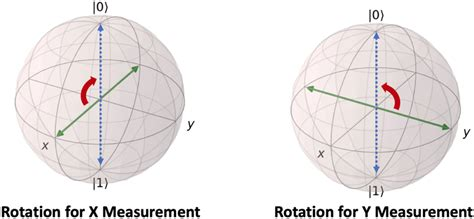
\includegraphics{figures/pauli_axes.jpeg}
\caption{Pauli rotations}
\end{figure}

\begin{center}\rule{0.5\linewidth}{0.5pt}\end{center}

    \begin{tcolorbox}[breakable, size=fbox, boxrule=1pt, pad at break*=1mm,colback=cellbackground, colframe=cellborder]
\prompt{In}{incolor}{4}{\boxspacing}
\begin{Verbatim}[commandchars=\\\{\}]
\PY{c+c1}{\PYZsh{}\PYZsh{}\PYZsh{}\PYZsh{} Python sandbox \PYZhy{} verify Pauli algebra}
\PY{k+kn}{import} \PY{n+nn}{numpy} \PY{k}{as} \PY{n+nn}{np}

\PY{n}{I} \PY{o}{=} \PY{n}{np}\PY{o}{.}\PY{n}{eye}\PY{p}{(}\PY{l+m+mi}{2}\PY{p}{,} \PY{n}{dtype}\PY{o}{=}\PY{n+nb}{complex}\PY{p}{)}
\PY{n}{X} \PY{o}{=} \PY{n}{np}\PY{o}{.}\PY{n}{array}\PY{p}{(}\PY{p}{[}\PY{p}{[}\PY{l+m+mi}{0}\PY{p}{,}\PY{l+m+mi}{1}\PY{p}{]}\PY{p}{,}\PY{p}{[}\PY{l+m+mi}{1}\PY{p}{,}\PY{l+m+mi}{0}\PY{p}{]}\PY{p}{]}\PY{p}{,} \PY{n}{dtype}\PY{o}{=}\PY{n+nb}{complex}\PY{p}{)}
\PY{n}{Y} \PY{o}{=} \PY{n}{np}\PY{o}{.}\PY{n}{array}\PY{p}{(}\PY{p}{[}\PY{p}{[}\PY{l+m+mi}{0}\PY{p}{,}\PY{o}{\PYZhy{}}\PY{l+m+mi}{1}\PY{n}{j}\PY{p}{]}\PY{p}{,}\PY{p}{[}\PY{l+m+mi}{1}\PY{n}{j}\PY{p}{,}\PY{l+m+mi}{0}\PY{p}{]}\PY{p}{]}\PY{p}{,} \PY{n}{dtype}\PY{o}{=}\PY{n+nb}{complex}\PY{p}{)}
\PY{n}{Z} \PY{o}{=} \PY{n}{np}\PY{o}{.}\PY{n}{array}\PY{p}{(}\PY{p}{[}\PY{p}{[}\PY{l+m+mi}{1}\PY{p}{,}\PY{l+m+mi}{0}\PY{p}{]}\PY{p}{,}\PY{p}{[}\PY{l+m+mi}{0}\PY{p}{,}\PY{o}{\PYZhy{}}\PY{l+m+mi}{1}\PY{p}{]}\PY{p}{]}\PY{p}{,} \PY{n}{dtype}\PY{o}{=}\PY{n+nb}{complex}\PY{p}{)}

\PY{k}{for} \PY{n}{name}\PY{p}{,} \PY{n}{P} \PY{o+ow}{in} \PY{p}{[}\PY{p}{(}\PY{l+s+s1}{\PYZsq{}}\PY{l+s+s1}{X}\PY{l+s+s1}{\PYZsq{}}\PY{p}{,}\PY{n}{X}\PY{p}{)}\PY{p}{,} \PY{p}{(}\PY{l+s+s1}{\PYZsq{}}\PY{l+s+s1}{Y}\PY{l+s+s1}{\PYZsq{}}\PY{p}{,}\PY{n}{Y}\PY{p}{)}\PY{p}{,} \PY{p}{(}\PY{l+s+s1}{\PYZsq{}}\PY{l+s+s1}{Z}\PY{l+s+s1}{\PYZsq{}}\PY{p}{,}\PY{n}{Z}\PY{p}{)}\PY{p}{]}\PY{p}{:}
    \PY{n+nb}{print}\PY{p}{(}\PY{l+s+sa}{f}\PY{l+s+s2}{\PYZdq{}}\PY{l+s+si}{\PYZob{}}\PY{n}{name}\PY{l+s+si}{\PYZcb{}}\PY{l+s+s2}{² == I ?}\PY{l+s+s2}{\PYZdq{}}\PY{p}{,} \PY{n}{np}\PY{o}{.}\PY{n}{allclose}\PY{p}{(}\PY{n}{P} \PY{o}{@} \PY{n}{P}\PY{p}{,} \PY{n}{I}\PY{p}{)}\PY{p}{)}
    \PY{n+nb}{print}\PY{p}{(}\PY{l+s+sa}{f}\PY{l+s+s2}{\PYZdq{}}\PY{l+s+si}{\PYZob{}}\PY{n}{name}\PY{l+s+si}{\PYZcb{}}\PY{l+s+s2}{† }\PY{l+s+si}{\PYZob{}}\PY{n}{name}\PY{l+s+si}{\PYZcb{}}\PY{l+s+s2}{ == I ?}\PY{l+s+s2}{\PYZdq{}}\PY{p}{,} \PY{n}{np}\PY{o}{.}\PY{n}{allclose}\PY{p}{(}\PY{n}{P}\PY{o}{.}\PY{n}{conj}\PY{p}{(}\PY{p}{)}\PY{o}{.}\PY{n}{T} \PY{o}{@} \PY{n}{P}\PY{p}{,} \PY{n}{I}\PY{p}{)}\PY{p}{)}

\PY{k+kn}{import} \PY{n+nn}{numpy} \PY{k}{as} \PY{n+nn}{np}
\PY{n}{I} \PY{o}{=} \PY{n}{np}\PY{o}{.}\PY{n}{eye}\PY{p}{(}\PY{l+m+mi}{2}\PY{p}{)}
\PY{n}{X} \PY{o}{=} \PY{n}{np}\PY{o}{.}\PY{n}{array}\PY{p}{(}\PY{p}{[}\PY{p}{[}\PY{l+m+mi}{0}\PY{p}{,}\PY{l+m+mi}{1}\PY{p}{]}\PY{p}{,}\PY{p}{[}\PY{l+m+mi}{1}\PY{p}{,}\PY{l+m+mi}{0}\PY{p}{]}\PY{p}{]}\PY{p}{)}
\PY{n}{Y} \PY{o}{=} \PY{n}{np}\PY{o}{.}\PY{n}{array}\PY{p}{(}\PY{p}{[}\PY{p}{[}\PY{l+m+mi}{0}\PY{p}{,}\PY{o}{\PYZhy{}}\PY{l+m+mi}{1}\PY{n}{j}\PY{p}{]}\PY{p}{,}\PY{p}{[}\PY{l+m+mi}{1}\PY{n}{j}\PY{p}{,}\PY{l+m+mi}{0}\PY{p}{]}\PY{p}{]}\PY{p}{)}
\PY{n}{Z} \PY{o}{=} \PY{n}{np}\PY{o}{.}\PY{n}{array}\PY{p}{(}\PY{p}{[}\PY{p}{[}\PY{l+m+mi}{1}\PY{p}{,}\PY{l+m+mi}{0}\PY{p}{]}\PY{p}{,}\PY{p}{[}\PY{l+m+mi}{0}\PY{p}{,}\PY{o}{\PYZhy{}}\PY{l+m+mi}{1}\PY{p}{]}\PY{p}{]}\PY{p}{)}
\end{Verbatim}
\end{tcolorbox}

    \begin{Verbatim}[commandchars=\\\{\}]
X² == I ? True
X† X == I ? True
Y² == I ? True
Y† Y == I ? True
Z² == I ? True
Z† Z == I ? True
    \end{Verbatim}

    Exercise: verify \(X^2=Y^2=Z^2=IX^2=Y^2=Z^2=I\).

\begin{verbatim}
Bloch‑sphere view — XX flips the sphere around the x‑axis, ZZ around z‑axis (see textbook figures pauli_x.png, pauli_z.png).
\end{verbatim}

    \hypertarget{inner-product-norm-orthogonality}{%
\subsection*{2.4\,Inner Product, Norm \&
Orthogonality}\label{inner-product-norm-orthogonality}}

The Dirac inner product, state normalisation and the geometric test for
orthogonality.

Inner products become measurement probabilities and kernel entries;
norms guarantee those probabilities sum to\,1 and ensure numerical
stability.

\begin{longtable}[]{@{}
  >{\raggedright\arraybackslash}p{(\columnwidth - 2\tabcolsep) * \real{0.4000}}
  >{\raggedright\arraybackslash}p{(\columnwidth - 2\tabcolsep) * \real{0.6000}}@{}}
\toprule\noalign{}
\begin{minipage}[b]{\linewidth}\raggedright
Code
\end{minipage} & \begin{minipage}[b]{\linewidth}\raggedright
Outcome
\end{minipage} \\
\midrule\noalign{}
\endhead
\bottomrule\noalign{}
\endlastfoot
\,2.4‑A & \textbf{compute} \(\langle v \lvert w\rangle\) for two
arbitrary complex vectors with a helper function. \\
\,2.4‑B & \textbf{determine} if two qubit states are orthogonal via the
inner product. \\
\,2.4‑C & \textbf{normalise} any non‑zero state vector to unit norm
using Python. \\
\end{longtable}

\begin{center}\rule{0.5\linewidth}{0.5pt}\end{center}

\hypertarget{dual-vector-in-dirac-braket-notation}{%
\subsubsection*{Dual Vector in Dirac (Bra--Ket)
Notation}\label{dual-vector-in-dirac-braket-notation}}

Given a ket\\
\[
\boxed{\;\lvert\psi\rangle \in \mathcal H\;}
\]\\
--- a column vector in the Hilbert space \(\mathcal H\) ---

its \textbf{dual vector} (or \textbf{bra}) is

\[
\boxed{\;\langle\psi\rvert \equiv \bigl(\lvert\psi\rangle\bigr)^{\dagger}\;}
\]

\begin{itemize}
\item
  \textbf{Mathematically:}\\
  \(\langle\psi|\) lives in the \textbf{dual space} \(\mathcal H^{*}\),
  the set of linear functionals that map kets to complex numbers.
\item
  \textbf{Operationally:}\\
  For any ket \(\lvert\phi\rangle\), \[
  \langle\psi\,|\,\phi\rangle
  = \mathrm{inner\;product}(\psi,\phi)
  \in \mathbb C .
  \]
\item
  \textbf{Matrix picture:}\\
  If \(\lvert\psi\rangle\) is the column vector
  \(\begin{pmatrix}\psi_0\\\psi_1\\\vdots\end{pmatrix}\), then\\
  \[
  \langle\psi\rvert = \bigl(\psi_0^{\!*},\;\psi_1^{\!*},\;\dots\bigr)
  \] --- i.e., the \textbf{conjugate‑transpose} (adjoint) of the ket.
\end{itemize}

Thus the bra \(\langle\psi|\) is the dual vector that, via the inner
product, turns any ket into a complex scalar.

\begin{center}\rule{0.5\linewidth}{0.5pt}\end{center}

\hypertarget{matrix-refresher-adjoint-conjugatetranspose-of-a-complex-matrix}{%
\paragraph{Matrix refresher Adjoint (Conjugate‑Transpose) of a Complex
Matrix}\label{matrix-refresher-adjoint-conjugatetranspose-of-a-complex-matrix}}

\textbf{Complex Conjugate}

For any complex number \(z = a + ib , \qquad a,b\in\mathbb R\), its
\textbf{conjugate} is \(z^{*} = a - ib\).

That is:

\begin{longtable}[]{@{}lll@{}}
\toprule\noalign{}
Component & Before conjugation & After conjugation \\
\midrule\noalign{}
\endhead
\bottomrule\noalign{}
\endlastfoot
Real part &  \( \operatorname{Re}(z)=a  \) & \textbf{unchanged} \\
Imag part &  \( \operatorname{Im}(z)=b  \) & \textbf{sign flips} →
\(-b\) \\
\end{longtable}

\textbf{Adjoint (Conjugate‑Transpose)}

For any complex matrix \(A \in \mathbb{C}^{m\times n}\), the
\textbf{adjoint}---also called the \textbf{Hermitian conjugate} or
\textbf{conjugate‑transpose}---is denoted \(A^{\dagger}\) and defined by

\[
\boxed{\;
A^{\dagger} \;=\; \bigl(A^{*}\bigr)^{\mathsf T}
\;}
\]

where

\begin{itemize}
\tightlist
\item
  \(A^{*}\) = element‑wise \textbf{complex conjugate} of \(A\)\\
\item
  \((\cdot)^{\mathsf T}\) = \textbf{transpose} operation (rows ↔
  columns).
\end{itemize}

Equivalently, the matrix elements satisfy

\[
\bigl(A^{\dagger}\bigr)_{ij} = \bigl(A_{ji}\bigr)^{*}.
\]

\hypertarget{key-properties}{%
\subparagraph{Key properties}\label{key-properties}}

\begin{itemize}
\tightlist
\item
  \(\bigl(A^{\dagger}\bigr)^{\dagger} = A\)\\
\item
  \((AB)^{\dagger} = B^{\dagger}A^{\dagger}\) (order reverses)\\
\item
  A matrix is \textbf{Hermitian} if \(A^{\dagger}=A\); \textbf{unitary}
  if \(A^{\dagger}A = I\).
\end{itemize}

    \begin{tcolorbox}[breakable, size=fbox, boxrule=1pt, pad at break*=1mm,colback=cellbackground, colframe=cellborder]
\prompt{In}{incolor}{5}{\boxspacing}
\begin{Verbatim}[commandchars=\\\{\}]
\PY{k+kn}{import} \PY{n+nn}{numpy} \PY{k}{as} \PY{n+nn}{np}

\PY{n}{A} \PY{o}{=} \PY{n}{np}\PY{o}{.}\PY{n}{array}\PY{p}{(}\PY{p}{[}\PY{p}{[}\PY{l+m+mi}{1}\PY{o}{+}\PY{l+m+mi}{2}\PY{n}{j}\PY{p}{,} \PY{l+m+mi}{3}\PY{o}{\PYZhy{}}\PY{l+m+mi}{1}\PY{n}{j}\PY{p}{]}\PY{p}{,}
              \PY{p}{[}\PY{l+m+mi}{4}\PY{o}{+}\PY{l+m+mi}{0}\PY{n}{j}\PY{p}{,} \PY{l+m+mi}{5}\PY{o}{+}\PY{l+m+mi}{5}\PY{n}{j}\PY{p}{]}\PY{p}{]}\PY{p}{)}

\PY{n}{A\PYZus{}dag} \PY{o}{=} \PY{n}{A}\PY{o}{.}\PY{n}{conj}\PY{p}{(}\PY{p}{)}\PY{o}{.}\PY{n}{T}    \PY{c+c1}{\PYZsh{} conjugate\PYZhy{}transpose}
\PY{n+nb}{print}\PY{p}{(}\PY{l+s+s2}{\PYZdq{}}\PY{l+s+s2}{A† =}\PY{l+s+se}{\PYZbs{}n}\PY{l+s+s2}{\PYZdq{}}\PY{p}{,} \PY{n}{A\PYZus{}dag}\PY{p}{)}
\end{Verbatim}
\end{tcolorbox}

    \begin{Verbatim}[commandchars=\\\{\}]
A† =
 [[1.-2.j 4.-0.j]
 [3.+1.j 5.-5.j]]
    \end{Verbatim}

    \begin{center}\rule{0.5\linewidth}{0.5pt}\end{center}

\hypertarget{dirac-inner-product}{%
\paragraph{Dirac Inner Product}\label{dirac-inner-product}}

Notation if inner product of two states : \(\langle v | w \rangle\) or
\((v,w)\).

For vectors \(v,w\in\mathbb C^{\,n}\)

\[
\boxed{\;
\langle v \,|\, w\rangle \;=\; v^{\dagger} w
\;=\; \sum_{k=1}^{n} v_k^{\!*}\,w_k
\;}
\]

\begin{itemize}
\tightlist
\item
  \textbf{Conjugate
  symmetry} \(\langle v|w\rangle = \langle w|v\rangle^{*}\)\\
\item
  \textbf{Linearity in the second
  slot} \(\langle v|(\alpha w+\beta u)\rangle = \alpha\,\langle v|w\rangle+\beta\,\langle v|u\rangle\)
\end{itemize}

(This makes \((\mathbb C^{n},\langle\cdot|\cdot\rangle)\) an
\textbf{inner‑product space}, also know as a \textbf{Hilbert Space}.)

\begin{center}\rule{0.5\linewidth}{0.5pt}\end{center}

\hypertarget{norm-length-and-normalisation}{%
\paragraph{Norm (Length) and
Normalisation}\label{norm-length-and-normalisation}}

\[
\|v\| \;=\; \sqrt{\langle v|v\rangle}
\]

A \textbf{quantum state‑vector} must satisfy \(\|v\|=1\). To normalise:

\[
\lvert\psi_{\text{norm}}\rangle = \frac{\lvert\psi\rangle}{\|\,\psi\|}
\]

\begin{center}\rule{0.5\linewidth}{0.5pt}\end{center}

\hypertarget{orthogonality}{%
\paragraph{Orthogonality}\label{orthogonality}}

Vectors \(v,w\) are \textbf{orthogonal} iff inner product is zero:

\[
\langle v | w\rangle = 0 .
\]

For qubits this means the measurement outcomes are perfectly
distinguishable.

\begin{itemize}
\tightlist
\item
  Verfy that \(\lvert w\rangle \equiv (1, 1)\) and
  \(\lvert v\rangle \equiv (1, -1)\) are orthogonal. \textgreater{} What
  are their normalised forms? ---
\end{itemize}

    \begin{tcolorbox}[breakable, size=fbox, boxrule=1pt, pad at break*=1mm,colback=cellbackground, colframe=cellborder]
\prompt{In}{incolor}{6}{\boxspacing}
\begin{Verbatim}[commandchars=\\\{\}]
\PY{c+c1}{\PYZsh{}\PYZsh{}\PYZsh{}\PYZsh{} Python demo \PYZhy{} inner product \PYZam{} normalisation}
\PY{k+kn}{import} \PY{n+nn}{numpy} \PY{k}{as} \PY{n+nn}{np}

\PY{k}{def} \PY{n+nf}{inner}\PY{p}{(}\PY{n}{v}\PY{p}{,} \PY{n}{w}\PY{p}{)}\PY{p}{:}
    \PY{k}{return} \PY{n}{np}\PY{o}{.}\PY{n}{vdot}\PY{p}{(}\PY{n}{v}\PY{p}{,} \PY{n}{w}\PY{p}{)}      \PY{c+c1}{\PYZsh{} conjugate dot product}

\PY{c+c1}{\PYZsh{} random 2D complex vectors}
\PY{n}{v} \PY{o}{=} \PY{n}{np}\PY{o}{.}\PY{n}{random}\PY{o}{.}\PY{n}{randn}\PY{p}{(}\PY{l+m+mi}{2}\PY{p}{)} \PY{o}{+} \PY{l+m+mi}{1}\PY{n}{j}\PY{o}{*}\PY{n}{np}\PY{o}{.}\PY{n}{random}\PY{o}{.}\PY{n}{randn}\PY{p}{(}\PY{l+m+mi}{2}\PY{p}{)}
\PY{n}{w} \PY{o}{=} \PY{n}{np}\PY{o}{.}\PY{n}{random}\PY{o}{.}\PY{n}{randn}\PY{p}{(}\PY{l+m+mi}{2}\PY{p}{)} \PY{o}{+} \PY{l+m+mi}{1}\PY{n}{j}\PY{o}{*}\PY{n}{np}\PY{o}{.}\PY{n}{random}\PY{o}{.}\PY{n}{randn}\PY{p}{(}\PY{l+m+mi}{2}\PY{p}{)}

\PY{n+nb}{print}\PY{p}{(}\PY{l+s+s2}{\PYZdq{}}\PY{l+s+s2}{⟨v|w⟩ =}\PY{l+s+s2}{\PYZdq{}}\PY{p}{,} \PY{n}{inner}\PY{p}{(}\PY{n}{v}\PY{p}{,} \PY{n}{w}\PY{p}{)}\PY{p}{)}

\PY{c+c1}{\PYZsh{} normalise v}
\PY{n}{v\PYZus{}norm} \PY{o}{=} \PY{n}{v} \PY{o}{/} \PY{n}{np}\PY{o}{.}\PY{n}{linalg}\PY{o}{.}\PY{n}{norm}\PY{p}{(}\PY{n}{v}\PY{p}{)}
\PY{n+nb}{print}\PY{p}{(}\PY{l+s+s2}{\PYZdq{}}\PY{l+s+s2}{‖v\PYZus{}norm‖² =}\PY{l+s+s2}{\PYZdq{}}\PY{p}{,} \PY{n}{inner}\PY{p}{(}\PY{n}{v\PYZus{}norm}\PY{p}{,} \PY{n}{v\PYZus{}norm}\PY{p}{)}\PY{o}{.}\PY{n}{real}\PY{p}{)}
\end{Verbatim}
\end{tcolorbox}

    \begin{Verbatim}[commandchars=\\\{\}]
⟨v|w⟩ = (0.6537321240532018-0.5177772916475541j)
‖v\_norm‖² = 0.9999999999999998
    \end{Verbatim}

    \begin{tcolorbox}[breakable, size=fbox, boxrule=1pt, pad at break*=1mm,colback=cellbackground, colframe=cellborder]
\prompt{In}{incolor}{7}{\boxspacing}
\begin{Verbatim}[commandchars=\\\{\}]
\PY{k}{def} \PY{n+nf}{inner}\PY{p}{(}\PY{n}{v}\PY{p}{,} \PY{n}{w}\PY{p}{)}\PY{p}{:}
    \PY{k}{return} \PY{n}{np}\PY{o}{.}\PY{n}{vdot}\PY{p}{(}\PY{n}{v}\PY{p}{,} \PY{n}{w}\PY{p}{)}     \PY{c+c1}{\PYZsh{} conjugate dot}
\PY{n}{v} \PY{o}{=} \PY{n}{np}\PY{o}{.}\PY{n}{array}\PY{p}{(}\PY{p}{[}\PY{l+m+mi}{1}\PY{p}{,}\PY{l+m+mi}{0}\PY{p}{]}\PY{p}{)}
\PY{n}{w} \PY{o}{=} \PY{n}{np}\PY{o}{.}\PY{n}{array}\PY{p}{(}\PY{p}{[}\PY{l+m+mi}{0}\PY{p}{,}\PY{l+m+mi}{1}\PY{p}{]}\PY{p}{)}
\PY{n+nb}{print}\PY{p}{(}\PY{l+s+sa}{f}\PY{l+s+s1}{\PYZsq{}}\PY{l+s+s1}{⟨v|w⟩ = }\PY{l+s+si}{\PYZob{}}\PY{n}{inner}\PY{p}{(}\PY{n}{v}\PY{p}{,}\PY{n}{w}\PY{p}{)}\PY{l+s+si}{\PYZcb{}}\PY{l+s+s1}{\PYZsq{}}\PY{p}{)}   \PY{c+c1}{\PYZsh{} 0  ⇒ orthogonal}
\end{Verbatim}
\end{tcolorbox}

    \begin{Verbatim}[commandchars=\\\{\}]
⟨v|w⟩ = 0
    \end{Verbatim}

    The state‑space with this inner product is a Hilbert space.

    \hypertarget{outer-product-completeness}{%
\subsection*{2.5\,Outer Product \&
Completeness}\label{outer-product-completeness}}

\begin{longtable}[]{@{}
  >{\raggedright\arraybackslash}p{(\columnwidth - 2\tabcolsep) * \real{0.4000}}
  >{\raggedright\arraybackslash}p{(\columnwidth - 2\tabcolsep) * \real{0.6000}}@{}}
\toprule\noalign{}
\begin{minipage}[b]{\linewidth}\raggedright
Code
\end{minipage} & \begin{minipage}[b]{\linewidth}\raggedright
Outcome
\end{minipage} \\
\midrule\noalign{}
\endhead
\bottomrule\noalign{}
\endlastfoot
\,2.5‑A & \textbf{generate} the outer product
\(\lvert v\rangle\langle w\rvert\) for two qubit states in code and
\textbf{interpret} it as a rank‑1 linear operator. \\
\,2.5‑B & \textbf{prove or verify} numerically that
\(\sum_{x\in\{0,1\}} \lvert x\rangle\langle x\rvert = I_{2}\)
(single‑qubit completeness). \\
\,2.5‑C & \textbf{extend} the completeness relation to two qubits and
\textbf{confirm} with a NumPy test. \\
\end{longtable}

\begin{itemize}
\item
  Building operators via vector outer product (dyadic products) and
  resolving the identity as a sum of projectors.
\item
  Enables density‑matrix notation, projective measurement theory and the
  ``insert\,\(I\)'' trick used in block‑encoding and swap‑test
  derivations.
\end{itemize}

\begin{center}\rule{0.5\linewidth}{0.5pt}\end{center}

\hypertarget{outer-dyadic-product}{%
\paragraph{Outer (Dyadic) Product}\label{outer-dyadic-product}}

Given kets \(\lvert v\rangle\) and \(\lvert w\rangle\) the \textbf{outer
product}

\[
\boxed{\;
\lvert v\rangle\langle w\rvert
\;}
\] is a \textbf{linear operator} acting on any \(\lvert u\rangle\) as

\[
\bigl(\lvert v\rangle\langle w\rvert\bigr)\lvert u\rangle
= \langle w|u\rangle \, \lvert v\rangle .
\]

\emph{Rank‑1 projector} when \(\lvert v\rangle=\lvert w\rangle\).

\textbf{Why the name ``dyadic''?}

In linear‑algebra literature (especially tensor analysis) a
\textbf{dyad} refers to a tensor formed from the tensor (outer) product
of two vectors;

Dirac's \(\lvert v\rangle\!\langle w\rvert\) is the quantum‑mechanics
version of that concept.

\begin{center}\rule{0.5\linewidth}{0.5pt}\end{center}

\hypertarget{projectors-measurement}{%
\paragraph{Projectors \& Measurement}\label{projectors-measurement}}

\begin{itemize}
\tightlist
\item
  Quantum measurements are described by a collection
  \(\lbrace M_m \rbrace\), where \(m\) refers to the outcomes that may
  occur.

  \begin{itemize}
  \tightlist
  \item
    \(p(m) = \langle \psi \lvert M_m^{\dagger} M_m \lvert \psi \rangle\)
  \item
    \(p(0) = \langle \psi \lvert M_0^{\dagger} M_0 \lvert \psi \rangle = \langle \psi \lvert M_0 \lvert \psi \rangle = \begin{bmatrix}a^*&b^*\end{bmatrix} \begin{bmatrix}1&0\\0&0\end{bmatrix} \begin{bmatrix}a\\b\end{bmatrix} = \lvert a \lvert ^2\)
  \end{itemize}
\item
  Projector onto state \(\lvert0\rangle\):
  \(M_0=\lvert0\rangle\langle0\rvert\).\\
\item
  Measuring a qubit in the computational basis applies \(M_0\)
  \textbf{or} \(M_1\) and renormalises, and the state becomes:

  \begin{itemize}
  \tightlist
  \item
     \(\frac{M_m \lvert \psi \rangle}{\sqrt{\langle\psi \lvert M_m^{\dagger} M_m \lvert \psi \rangle }}
     \)
  \item
    \(\frac{M_0 \lvert \psi \rangle}{\lvert a \lvert} = \frac{a}{\lvert a \lvert} \lvert0 \rangle\)
  \end{itemize}
\end{itemize}

\begin{center}\rule{0.5\linewidth}{0.5pt}\end{center}

\hypertarget{completeness-resolution-of-identity}{%
\paragraph{Completeness (Resolution of
Identity)}\label{completeness-resolution-of-identity}}

For any orthonormal basis \(\{\lvert e_k\rangle\}\):

\[
\boxed{\;
\sum_{k} \lvert e_k\rangle\langle e_k\rvert = I
\;}
\]

Single qubit:

\[
\lvert0\rangle\langle0\rvert + \lvert1\rangle\langle1\rvert
= \begin{bmatrix}1\\0\end{bmatrix} \begin{bmatrix}1&0\end{bmatrix} + \begin{bmatrix}0\\1\end{bmatrix} \begin{bmatrix}0&1\end{bmatrix}
= \begin{bmatrix}1&0\\0&0\end{bmatrix} + \begin{bmatrix}0&0\\0&1\end{bmatrix}  
= \begin{bmatrix}1&0\\0&1\end{bmatrix} = I_{2}.
\]

Two qubits:

\[
\sum_{x\in\{0,1\}^{2}} \lvert x\rangle\langle x\rvert
= \lvert00\rangle\langle00\rvert+\dots+\lvert11\rangle\langle11\rvert
= I_{4}.
\]

\begin{itemize}
\tightlist
\item
  Measurment operators satisfy the completeness equation.
\end{itemize}

\begin{center}\rule{0.5\linewidth}{0.5pt}\end{center}

    \begin{tcolorbox}[breakable, size=fbox, boxrule=1pt, pad at break*=1mm,colback=cellbackground, colframe=cellborder]
\prompt{In}{incolor}{8}{\boxspacing}
\begin{Verbatim}[commandchars=\\\{\}]
\PY{c+c1}{\PYZsh{}\PYZsh{}\PYZsh{}\PYZsh{} Python demo \PYZhy{} build projectors \PYZam{} verify completeness}
\PY{k+kn}{import} \PY{n+nn}{numpy} \PY{k}{as} \PY{n+nn}{np}

\PY{c+c1}{\PYZsh{} basis kets}
\PY{n}{e0} \PY{o}{=} \PY{n}{np}\PY{o}{.}\PY{n}{array}\PY{p}{(}\PY{p}{[}\PY{p}{[}\PY{l+m+mi}{1}\PY{p}{]}\PY{p}{,}\PY{p}{[}\PY{l+m+mi}{0}\PY{p}{]}\PY{p}{]}\PY{p}{,} \PY{n}{dtype}\PY{o}{=}\PY{n+nb}{complex}\PY{p}{)}
\PY{n}{e1} \PY{o}{=} \PY{n}{np}\PY{o}{.}\PY{n}{array}\PY{p}{(}\PY{p}{[}\PY{p}{[}\PY{l+m+mi}{0}\PY{p}{]}\PY{p}{,}\PY{p}{[}\PY{l+m+mi}{1}\PY{p}{]}\PY{p}{]}\PY{p}{,} \PY{n}{dtype}\PY{o}{=}\PY{n+nb}{complex}\PY{p}{)}

\PY{n}{P0} \PY{o}{=} \PY{n}{e0} \PY{o}{@} \PY{n}{e0}\PY{o}{.}\PY{n}{T}\PY{o}{.}\PY{n}{conj}\PY{p}{(}\PY{p}{)}   \PY{c+c1}{\PYZsh{} \PYZbs{}lvert0\PYZbs{}rangle\PYZlt{}0|}
\PY{n}{P1} \PY{o}{=} \PY{n}{e1} \PY{o}{@} \PY{n}{e1}\PY{o}{.}\PY{n}{T}\PY{o}{.}\PY{n}{conj}\PY{p}{(}\PY{p}{)}   \PY{c+c1}{\PYZsh{} \PYZbs{}lvert1\PYZbs{}rangle\PYZlt{}1|}
\PY{n}{I2} \PY{o}{=} \PY{n}{P0} \PY{o}{+} \PY{n}{P1}

\PY{n+nb}{print}\PY{p}{(}\PY{l+s+s2}{\PYZdq{}}\PY{l+s+s2}{Projector P0 =}\PY{l+s+se}{\PYZbs{}n}\PY{l+s+s2}{\PYZdq{}}\PY{p}{,} \PY{n}{P0}\PY{p}{)}
\PY{n+nb}{print}\PY{p}{(}\PY{l+s+s2}{\PYZdq{}}\PY{l+s+s2}{Completeness check (I2):}\PY{l+s+se}{\PYZbs{}n}\PY{l+s+s2}{\PYZdq{}}\PY{p}{,} \PY{n}{I2}\PY{p}{)}


\PY{n}{I2} \PY{o}{=} \PY{n+nb}{sum}\PY{p}{(}\PY{n}{np}\PY{o}{.}\PY{n}{outer}\PY{p}{(}\PY{n}{b}\PY{p}{,}\PY{n}{b}\PY{p}{)} \PY{k}{for} \PY{n}{b} \PY{o+ow}{in} \PY{p}{[}\PY{n}{v}\PY{p}{,}\PY{n}{w}\PY{p}{]}\PY{p}{)}  \PY{c+c1}{\PYZsh{} v=\PYZbs{}lvert0\PYZbs{}rangle, w=\PYZbs{}lvert1\PYZbs{}rangle}
\PY{n+nb}{print}\PY{p}{(}\PY{n}{I2}\PY{p}{)}
\end{Verbatim}
\end{tcolorbox}

    \begin{Verbatim}[commandchars=\\\{\}]
Projector P0 =
 [[1.+0.j 0.+0.j]
 [0.+0.j 0.+0.j]]
Completeness check (I2):
 [[1.+0.j 0.+0.j]
 [0.+0.j 1.+0.j]]
[[1 0]
 [0 1]]
    \end{Verbatim}

    Quick sanity check in Python

    \begin{tcolorbox}[breakable, size=fbox, boxrule=1pt, pad at break*=1mm,colback=cellbackground, colframe=cellborder]
\prompt{In}{incolor}{9}{\boxspacing}
\begin{Verbatim}[commandchars=\\\{\}]
\PY{c+c1}{\PYZsh{} random normalised qubit state}
\PY{n}{np}\PY{o}{.}\PY{n}{random}\PY{o}{.}\PY{n}{seed}\PY{p}{(}\PY{l+m+mi}{0}\PY{p}{)}
\PY{n}{psi} \PY{o}{=} \PY{n}{np}\PY{o}{.}\PY{n}{random}\PY{o}{.}\PY{n}{randn}\PY{p}{(}\PY{l+m+mi}{2}\PY{p}{)} \PY{o}{+} \PY{l+m+mi}{1}\PY{n}{j}\PY{o}{*}\PY{n}{np}\PY{o}{.}\PY{n}{random}\PY{o}{.}\PY{n}{randn}\PY{p}{(}\PY{l+m+mi}{2}\PY{p}{)}
\PY{n}{psi} \PY{o}{/}\PY{o}{=} \PY{n}{np}\PY{o}{.}\PY{n}{linalg}\PY{o}{.}\PY{n}{norm}\PY{p}{(}\PY{n}{psi}\PY{p}{)}

\PY{c+c1}{\PYZsh{} verify probability sum to 1}
\PY{n}{probs} \PY{o}{=} \PY{n}{np}\PY{o}{.}\PY{n}{abs}\PY{p}{(}\PY{n}{psi}\PY{p}{)}\PY{o}{*}\PY{o}{*}\PY{l+m+mi}{2}
\PY{n+nb}{print}\PY{p}{(}\PY{l+s+s2}{\PYZdq{}}\PY{l+s+s2}{Probabilities:}\PY{l+s+s2}{\PYZdq{}}\PY{p}{,} \PY{n}{probs}\PY{p}{,} \PY{l+s+s2}{\PYZdq{}}\PY{l+s+s2}{sum:}\PY{l+s+s2}{\PYZdq{}}\PY{p}{,} \PY{n}{probs}\PY{o}{.}\PY{n}{sum}\PY{p}{(}\PY{p}{)}\PY{p}{)}
\end{Verbatim}
\end{tcolorbox}

    \begin{Verbatim}[commandchars=\\\{\}]
Probabilities: [0.43990623 0.56009377] sum: 0.9999999999999998
    \end{Verbatim}

    \hypertarget{where-were-headed}{%
\subsection*{2.6 Where We're Headed}\label{where-were-headed}}

Connecting the toolkit to unitary evolution, block‑encodings, quantum
kernels and OC‑SVM workflows.

Gives students a roadmap: each algebraic concept they master today
reappears as a lever in real algorithms and the final capstone project.

\hypertarget{how-these-outcomes-support-downstream-units}{%
\subsubsection*{How these outcomes support downstream
units}\label{how-these-outcomes-support-downstream-units}}

\begin{longtable}[]{@{}
  >{\raggedright\arraybackslash}p{(\columnwidth - 2\tabcolsep) * \real{0.4423}}
  >{\raggedright\arraybackslash}p{(\columnwidth - 2\tabcolsep) * \real{0.5577}}@{}}
\toprule\noalign{}
\begin{minipage}[b]{\linewidth}\raggedright
Toolkit Outcome Block
\end{minipage} & \begin{minipage}[b]{\linewidth}\raggedright
Enables later ability in \ldots{}
\end{minipage} \\
\midrule\noalign{}
\endhead
\bottomrule\noalign{}
\endlastfoot
2.0‑B,\,2.0‑C & Constructing and visualising \textbf{feature‑map states}
for quantum kernels (Unit\,4). \\
2.1‑B,\,2.1‑C & Counting Hilbert‑space dimension when doing
\textbf{complexity estimates} for block‑encodings. \\
2.2‑B & Proving \textbf{linear independence} of Pauli strings in
error‑correction (Unit\,2.5). \\
2.3‑B & Implementing \textbf{swap‑test circuits} (needs Pauli matrices
for measurement bases). \\
2.4‑A\ldots C & Calculating \textbf{kernel inner products} and
normalising support‑vector coefficients. \\
2.5‑A\ldots C & Building the \textbf{resolution‑of‑identity} step in
block‑encoding proofs (Unit\,3+). \\
\end{longtable}

This toolkit equips us for:

\begin{itemize}
\item
  Unitary evolution \(U^{\dagger}U=IU^{\dagger}U=I\) \(\rightarrow\)
  reversibility
\item
  Block‑encodings (non‑unitary \(A\) embedded in a bigger unitary \(U\))
\item
  Quantum kernels \& OC‑SVM (swap‑test = inner product circuit)
\end{itemize}

